\chapter{Week2-2 Nucleic Acid Structure}

\begin{introduction}
    \item 
\end{introduction}

\hypertarget{component}{%
\section{Components}\label{component}}

\begin{itemize}
\item
pentose (difference)
\item
base
\item
phosphate (phosphoester bond)
\end{itemize}

\hypertarget{conformation}{%
\section{conformation}\label{conformation}}

\begin{itemize}
\item
bases point inwards
\item
plots of torsion angle

\begin{itemize}
	\item
	main chain: extended (trans, \ang{180})
	\item
	\(\chi\): anti (\ang{0})
\end{itemize}

\begin{figure}
	\centering
	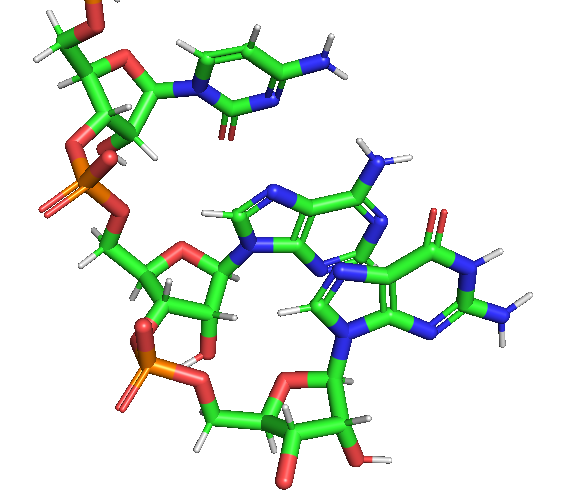
\includegraphics[width=0.5\linewidth]{E:/undergraduate_study/study/abroad study/2021 NUS/study/LSM3243/notes/2_3.png}
%	\caption{2\_3}
\end{figure}
\end{itemize}

\hypertarget{secondary-structure}{%
\section{Secondary structure}\label{secondary-structure}}

\hypertarget{double-helix}{%
\subsubsection{double helix}\label{double-helix}}

\begin{longtable}[]{@{}lll@{}}
\toprule
helix & (B) DNA & (\(\alpha\)) protein\tabularnewline
\midrule
\endhead
units per turn & 10.5 (10) & 3.6\tabularnewline
degree per unit & \ang{36} & \ang{100}\tabularnewline
rise per unit/nm & 0.34 &\tabularnewline
diameter/nm & 22 &\tabularnewline
\bottomrule
\end{longtable}

\hypertarget{grooves}{%
\subsection{grooves}\label{grooves}}

\begin{figure}
\centering
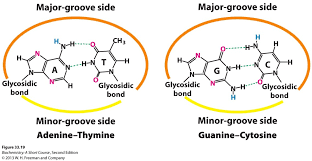
\includegraphics[width=0.7\linewidth]{2_4.png}
%\caption{2\_4}
\end{figure}

\begin{longtable}[]{@{}lll@{}}
\toprule
grooves & major & minor\tabularnewline
\midrule
\endhead
part of base & more & less\tabularnewline
actual H bonds & fewer & more\tabularnewline
bind & proteins & drugs\tabularnewline
\bottomrule
\end{longtable}

Most proteins perform non-sequence-specific binding, switching on/off
gene expression.

\hypertarget{forces-to-stablize}{%
\section{Forces to stablize}\label{forces-to-stablize}}

\hypertarget{hydrogen-bond-2}{%
\subsection{hydrogen bond}\label{hydrogen-bond-2}}

Waston-Crick base pairs vs unusual pairs

fraction of GC \(\to\) melting temperature. AT: local unwinding

\hypertarget{stacking-interaction}{%
\subsection{stacking interaction}\label{stacking-interaction}}

\begin{figure}
\centering
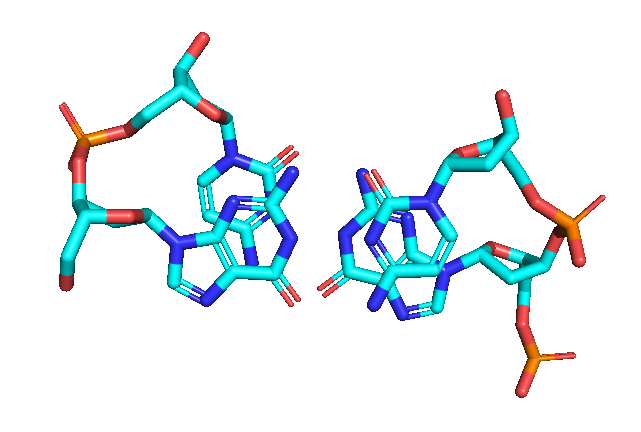
\includegraphics[width=0.6\linewidth]{E:/undergraduate_study/study/abroad study/2021 NUS/study/LSM3243/notes/2_7-2.png}
\caption*{GC superimposition}
\end{figure}

is a conbination of

\begin{itemize}
\item
vdW, where 0.34 nm is the optimal distance
\item
dipole-dipole, same direction \(\Leftrightarrow\) repel
\end{itemize}

bases on the next level rotate \ang{36} as a balance

\hypertarget{electrostatic-interaction}{%
\subsection{electrostatic interaction}\label{electrostatic-interaction}}

negative charged (-1 per bp) phosphate backbone: repulsion, controls
distance between two strands

\begin{itemize}
\item
low-salt: (phosphates) try to be trans; bases farther, prefer single
strand (PCR)
\item
high-salt: shield them to form double strand DNA
\end{itemize}

DNA prefers to take helix to 1) form stacking 2) avoid repulsion

\hypertarget{with-water}{%
\subsection{with water}\label{with-water}}

Water forms H bond with bases, pentoses and phosphate groups. The major
and minor grooves potentially form same amount of H bonds. But due to
larger space, the major groove needs more water molecules. This is the
cause of \textbf{entropy loss}.

As a result, the minor groove forms \textbf{more H bonds} with water,
i.e. more enthalpy gain. Thus, it can trap more water molecules (a
cluster that may not form H bonds) and compensate the entropy loss. In
contrast, the major groove only maintains one shallow layer of water.

\begin{figure}
\centering
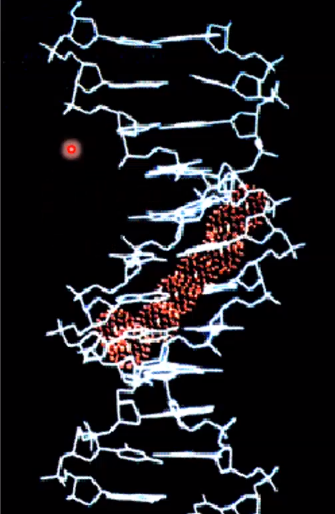
\includegraphics[width=0.4\linewidth]{E:/undergraduate_study/study/abroad study/2021 NUS/study/LSM3243/notes/2_8.png}
\caption*{spine of hydration}
\end{figure}

\hypertarget{other}{%
\section{other}\label{other}}

\begin{itemize}
\item
tightness: Z form (left-handed, seq-specific)\textgreater{}A form
(seq-specific/RNA, high salt)\textgreater{}B form (normal)
\item
RNA structure
\end{itemize}

\hypertarget{week3-1-hw}{%
\subsection{Week3-1 HW}\label{week3-1-hw}}

\begin{enumerate}
\def\labelenumi{\arabic{enumi}.}
\item
interactions

\begin{longtable}[]{@{}lll@{}}
	\toprule
	& protein & nucleic acid\tabularnewline
	\midrule
	\endhead
	interactions & \vtop{\hbox{\strut covalent bond
			(disulfide)}\hbox{\strut electrostatic (ion and
			dipole)}\hbox{\strut vdW}\hbox{\strut H
			bond}\hbox{\strut hydrophobic}} & \vtop{\hbox{\strut covalent
			bond}\hbox{\strut H bond}\hbox{\strut stacking (vdW,
			hydrophobic)}\hbox{\strut electrostatic}}\tabularnewline
	secondary & \textbf{H bond} & \textbf{H bond}
	(stacking)\tabularnewline
	tertiary & H bond, \textbf{hydrophobic} & H bond,
	\textbf{stacking}\tabularnewline
	\bottomrule
\end{longtable}
\item
effect of heat and salt on DNA?

salt stablizes the backbone, pushing the phosphate groups nearer and
thus harder to be denatured by heat.

a multi-layer structure:

\begin{figure}
	\centering
	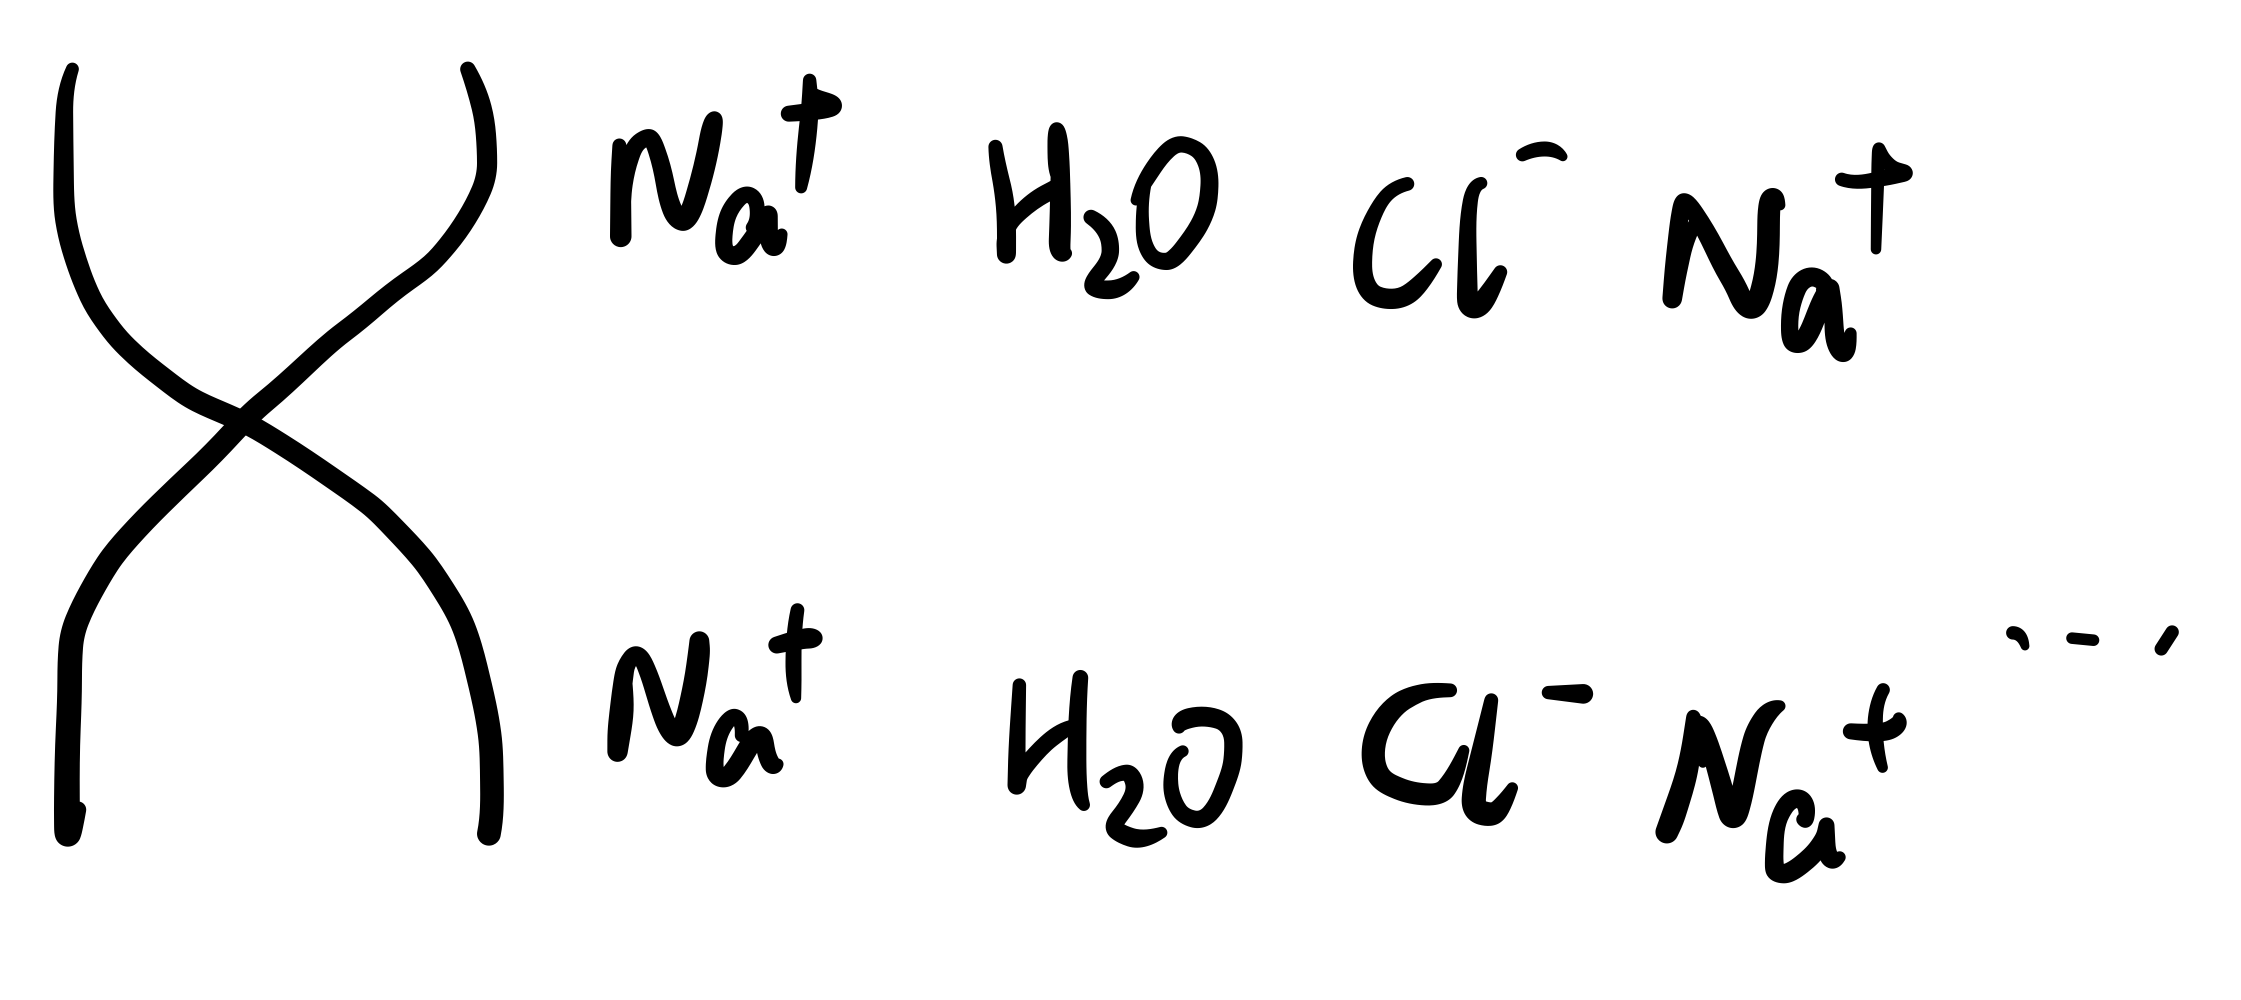
\includegraphics[width=0.5\linewidth]{E:/undergraduate_study/study/abroad study/2021 NUS/study/LSM3243/notes/2_9.png}
\end{figure}

\end{enumerate}
